\documentclass[tikz,border=12pt]{standalone}
\usepackage[T1]{fontenc}
\usepackage{mathpazo}
\usepackage{amsmath,amssymb}
\usetikzlibrary{arrows.meta, positioning, calc}

\definecolor{stblue}{HTML}{7B97AD}
\definecolor{rwgold}{HTML}{B8995E}
\definecolor{sage}{HTML}{7A9A7E}
\definecolor{dkbrown}{HTML}{3D3530}
\definecolor{wmgray}{HTML}{7B7067}
\definecolor{cream}{HTML}{F9F6F0}
\definecolor{border}{HTML}{D4C9B8}
\definecolor{terracotta}{HTML}{C47A6A}

\begin{document}
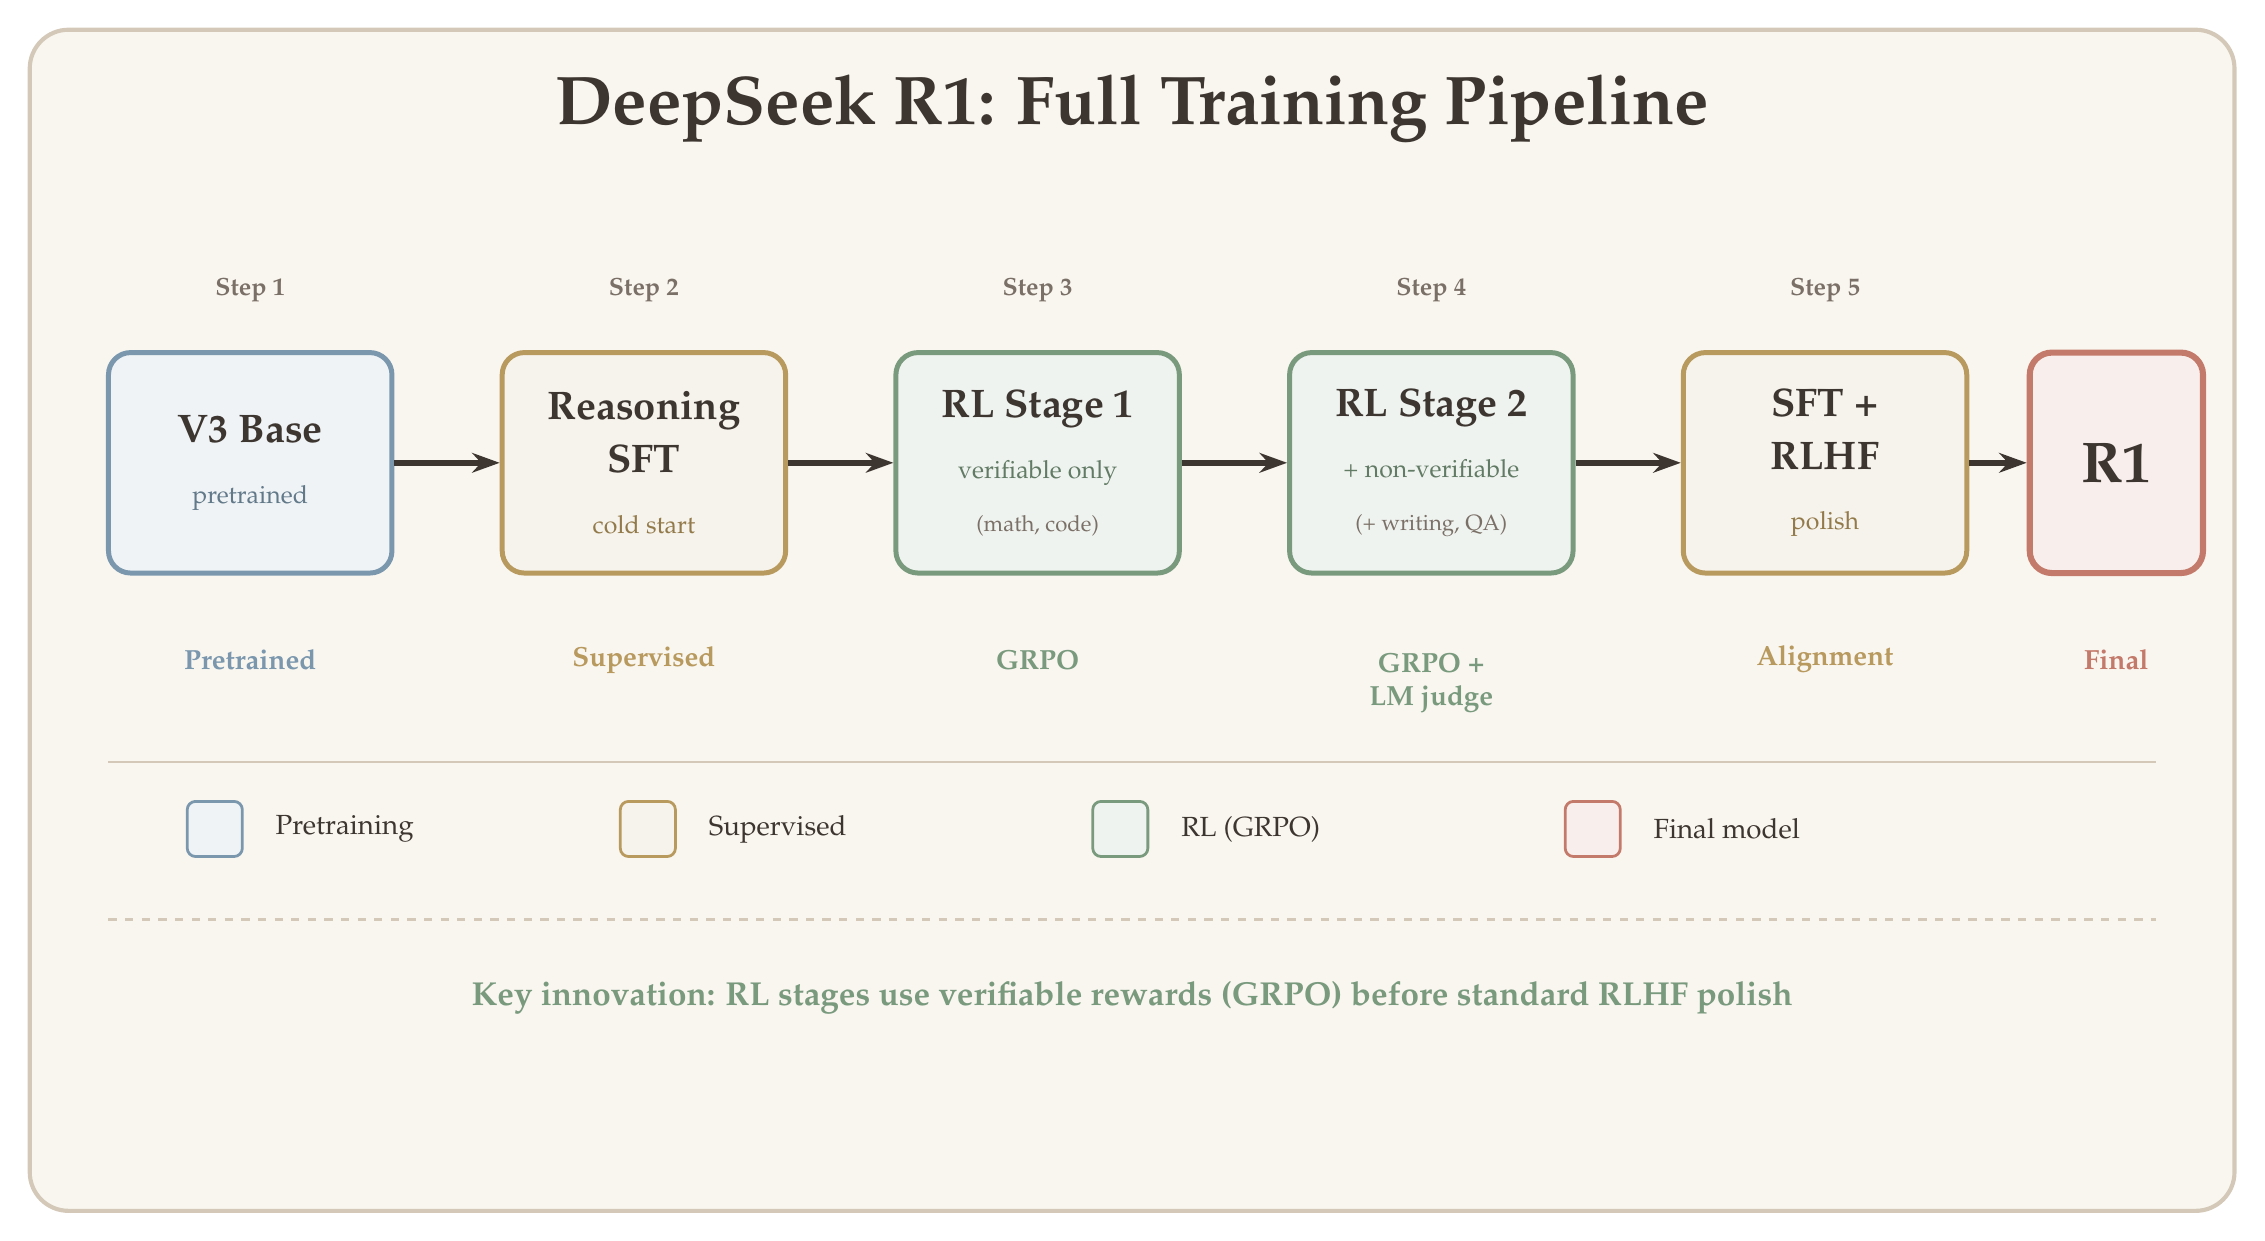
\begin{tikzpicture}[
  >={Stealth[length=3.5mm, width=2.5mm]},
  stagebox/.style 2 args={
    draw=#1, line width=1.8pt, fill=#1!12, rounded corners=8pt,
    minimum width=36mm, minimum height=28mm, font=\Large,
    text=dkbrown, align=center, inner sep=6pt
  },
  arr/.style={->, line width=2.2pt, dkbrown},
  note/.style={font=\normalsize, text=wmgray, align=center},
  stageann/.style={font=\normalsize\bfseries, align=center},
]

% Background
\fill[cream, rounded corners=14pt] (-1,-4.5) rectangle (27,10.5);
\draw[border, rounded corners=14pt, line width=1.5pt] (-1,-4.5) rectangle (27,10.5);

% Title
\node[font=\Huge\bfseries, text=dkbrown] at (13,9.5)
  {DeepSeek R1: Full Training Pipeline};

% ---- Stage boxes ----
% Box 1: V3 Base
\node[stagebox={stblue}{}] (s1) at (1.8,5)
  {\textbf{V3 Base}\\[4pt]
   \small\color{stblue!80!black} pretrained};

% Box 2: Reasoning SFT
\node[stagebox={rwgold}{}] (s2) at (6.8,5)
  {\textbf{Reasoning}\\[1pt]\textbf{SFT}\\[4pt]
   \small\color{rwgold!80!black} cold start};

% Box 3: RL Stage 1
\node[stagebox={sage}{}] (s3) at (11.8,5)
  {\textbf{RL Stage 1}\\[4pt]
   \small\color{sage!80!black} verifiable only\\[1pt]
   \footnotesize\color{wmgray} (math, code)};

% Box 4: RL Stage 2
\node[stagebox={sage}{}] (s4) at (16.8,5)
  {\textbf{RL Stage 2}\\[4pt]
   \small\color{sage!80!black} + non-verifiable\\[1pt]
   \footnotesize\color{wmgray} (+ writing, QA)};

% Box 5: SFT + RLHF
\node[stagebox={rwgold}{}] (s5) at (21.8,5)
  {\textbf{SFT +}\\[1pt]\textbf{RLHF}\\[4pt]
   \small\color{rwgold!80!black} polish};

% Box 6: R1
\node[draw=terracotta, line width=2.2pt, fill=terracotta!12, rounded corners=8pt,
  minimum width=22mm, minimum height=28mm, font=\huge\bfseries,
  text=dkbrown, align=center, inner sep=6pt]
  (s6) at (25.5,5)
  {\textbf{R1}};

% ---- Arrows between stages ----
\draw[arr] (s1.east) -- (s2.west);
\draw[arr] (s2.east) -- (s3.west);
\draw[arr] (s3.east) -- (s4.west);
\draw[arr] (s4.east) -- (s5.west);
\draw[arr] (s5.east) -- (s6.west);

% ---- Stage annotations below boxes ----
\node[stageann, text=stblue] at (1.8,2.5) {Pretrained};
\node[stageann, text=rwgold] at (6.8,2.5) {Supervised};
\node[stageann, text=sage]   at (11.8,2.5) {GRPO};
\node[stageann, text=sage]   at (16.8,2.2) {GRPO +\\LM judge};
\node[stageann, text=rwgold] at (21.8,2.5) {Alignment};
\node[stageann, text=terracotta] at (25.5,2.5) {Final};

% ---- Divider ----
\draw[border, line width=1pt] (0,1.2) -- (26,1.2);

% ---- Color legend ----
\fill[stblue!12, draw=stblue, line width=1pt, rounded corners=3pt]
  (1,0) rectangle (1.7,0.7);
\node[font=\normalsize, text=dkbrown, anchor=west] at (2,0.35)
  {Pretraining};

\fill[rwgold!12, draw=rwgold, line width=1pt, rounded corners=3pt]
  (6.5,0) rectangle (7.2,0.7);
\node[font=\normalsize, text=dkbrown, anchor=west] at (7.5,0.35)
  {Supervised};

\fill[sage!12, draw=sage, line width=1pt, rounded corners=3pt]
  (12.5,0) rectangle (13.2,0.7);
\node[font=\normalsize, text=dkbrown, anchor=west] at (13.5,0.35)
  {RL (GRPO)};

\fill[terracotta!12, draw=terracotta, line width=1pt, rounded corners=3pt]
  (18.5,0) rectangle (19.2,0.7);
\node[font=\normalsize, text=dkbrown, anchor=west] at (19.5,0.35)
  {Final model};

% ---- Bottom annotation ----
\draw[border, line width=0.8pt, dashed] (0,-0.8) -- (26,-0.8);
\node[font=\large\bfseries, text=sage] at (13,-1.8)
  {Key innovation: RL stages use verifiable rewards (GRPO) before standard RLHF polish};

% ---- Step numbers ----
\node[font=\small\bfseries, text=wmgray] at (1.8,7.2) {Step 1};
\node[font=\small\bfseries, text=wmgray] at (6.8,7.2) {Step 2};
\node[font=\small\bfseries, text=wmgray] at (11.8,7.2) {Step 3};
\node[font=\small\bfseries, text=wmgray] at (16.8,7.2) {Step 4};
\node[font=\small\bfseries, text=wmgray] at (21.8,7.2) {Step 5};

\end{tikzpicture}
\end{document}
